\documentclass[tikz,border=10pt]{standalone}
\begin{document}
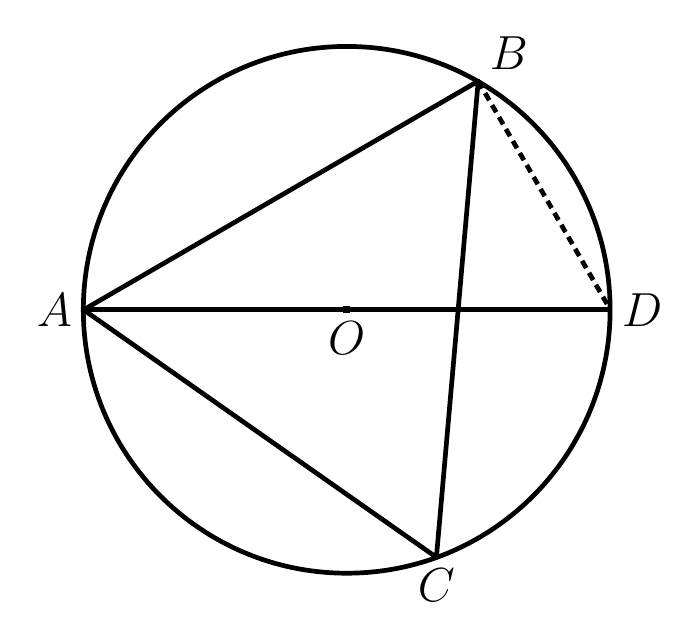
\begin{tikzpicture}[line width=1.7pt, line join=round]
  % Coordinates: origin at circle centre O, scale s = 0.021277 cm/px, y flipped
  \coordinate (O) at (0,0);
  \coordinate (A) at (-3.342,0);
  \coordinate (D) at (3.349,0);
  \coordinate (B) at (1.670,2.904);
  \coordinate (C) at (1.139,-3.143);

  % Circle, radius 157.24 px
  \draw (O) circle[radius=3.345];

  % Diameter AD (solid)
  \draw (A) -- (D);

  % Triangle ABC (solid sides AB, BC, CA)
  \draw (A) -- (B) -- (C) -- (A);

  % Chord BD (dashed), longer dashes: 3pt on, 2pt off
  \draw[dash pattern=on 3pt off 2pt] (B) -- (D);

  % Filled square marker at centre (O is at origin, so no calc needed), 2.5pt side
  \fill (-1.25pt,-1.25pt) rectangle (1.25pt,1.25pt);

  % Labels
  \node[font=\fontsize{17.5}{21}\selectfont, left]        at (A) {$A$};
  \node[font=\fontsize{17.5}{21}\selectfont, right]       at (D) {$D$};
  \node[font=\fontsize{17.5}{21}\selectfont, above right] at (B) {$B$};
  \node[font=\fontsize{17.5}{21}\selectfont, below]       at (C) {$C$};
  \node[font=\fontsize{17.5}{21}\selectfont, below]       at (O) {$O$};
\end{tikzpicture}
\end{document}